\section{The second family and the tight state \texorpdfstring{$\td$}{}}\label{sec:family}

Theorem~\ref{thm:pass} leaves the pulling problem in an unusual position. At the regular pentagon the gradient of the core length is the exact vector $\nabla\core=\frac12\mathbf1$ of Proposition~\ref{prop:gradpent}, and it lies in no subcone of the active wall gradients in either taco branch; the direction that certifies this keeps the four walls $w_1,w_4,w_5,w_6$ at equality while opening $w_7,w_8,w_9,w_{10}$ into the feasible side. Pulling therefore does not stop at the folklore state: it continues along the locus on which those four equalities persist,
\begin{equation}\label{eq:family}
  \mathcal E=\bigl\{\theta\in\overline{\M}\ :\ w_1(\theta)=w_4(\theta)=w_5(\theta)=w_6(\theta)=0\bigr\},
\end{equation}
the second mirror-symmetric one-parameter family of Proposition~\ref{prop:families}. This section follows $\mathcal E$ to its end.

The outcome is a single point $\td$, and every quantity associated with it is algebraic over one number field: its coordinates, the multipliers that block further pulling, and the curvature that makes the block strict all lie in a degree-twelve extension of $\Q$, so the entire optimality analysis can be carried out by exact arithmetic rather than approximation. At the same time, the field is not solvable by radicals: the splitting field of the defining sextic for $(x^\dagger)^2$ has Galois group $S_6$, so the tight state of Definition~\ref{def:pull} admits no radical expression, its $x$-coordinate already having none.

\subsection{Reduction to a plane curve}

\begin{proposition}[Family reduction]\label{prop:familyreduction}
On the mirror-symmetric component of $\mathcal E$ through $P^*$ and $\td$, the coordinates satisfy the identities
\begin{equation}\label{eq:familyids}
  g=\frac{1-x^2}{2x},\qquad a=h,\qquad b=g+x=\frac{x^2+1}{2x},\qquad \core=g+h+x=h+b,
\end{equation}
and the residual relation between the two remaining coordinates is the plane algebraic curve
\begin{equation}\label{eq:n5}
  N_5(x,h)=8h^3x^3+4h^2x^4+4h^2x^2+2hx^5-4hx^3-6hx+x^6+3x^4+3x^2+1=0 .
\end{equation}
Consequently this geometric family is represented by the selected real branch of $\{N_5=0\}$ with the positive chart and feasibility conditions retained, and on it the objective becomes a single-variable function: we abbreviate $\ell(x):=\core(c(x))$ for the restriction of the core length to the family curve $c(x)=\bigl(x,g(x),h(x),h(x),b(x)\bigr)$, so that
\begin{equation}\label{eq:ellofx}
  \ell(x)=h(x)+\frac{x^2+1}{2x} .
\end{equation}
\end{proposition}

\begin{proof}
The first wall admits the exact polynomial representative $2gx+x^2-1$, a positive multiple of $w_1$ on the branch, so for $x>0$ the equation $w_1=0$ is equivalent to $g=(1-x^2)/(2x)$. The mirror symmetry recorded in Proposition~\ref{prop:families} survives along $\mathcal E$ and identifies $a$ with $h$; it also exchanges the two core segments, so they have equal length. Since $M_1=(-x/2,\frac12)$ and $M_2=(\frac{g+h}2,\frac12)$ lie on a common horizontal line, the first core segment has length $(g+h+x)/2$ by Proposition~\ref{prop:nointerior}, whence $\core=g+h+x$. Eliminating the reflected data from the two remaining wall equations---a sequence of polynomial divisions verified by exact arithmetic in the ancillary suite \cite{anc}---leaves the identity $b=g+x$, which turns $\core=g+h+x$ into $\core=h+b$ and, with the value of $g$ already found, into $b=(x^2+1)/(2x)$; and it leaves exactly one further relation between $x$ and $h$, namely \eqref{eq:n5}.
\end{proof}

\begin{proposition}[Irreducibility of the family curve]\label{prop:n5irred}
The polynomial $N_5$ is irreducible over $\Q$. Polynomial identities established modulo $N_5$ therefore hold on its algebraic zero set; rational identities also require nonzero denominators. This does not identify all real points of that curve with valid folded states. We use only the real branch through $(x^\dagger,h^\dagger)$ and the pentagon, isolated in a rational height interval at an interior point and continued over $[x^\dagger,x_0]$ by the root-free certificates in Remark~\ref{rem:edge}.
\end{proposition}

\begin{proof}
Irreducibility is a finite computation with integer coefficients, verified by exact arithmetic in the ancillary suite \cite{anc}. The quotient $\Q[x,h]/(N_5)$ is then a domain. Remainder-zero computations establish the stated algebraic identities, while the interval and resultant certificates separately select the real branch and retain its geometric inequalities. Irreducibility alone says nothing about uniqueness of the real ordinate: at $x=1/5$, for example, the cubic $N_5(x,h)$ has three real roots.
\end{proof}

\subsection{Existence and exact identification}

\begin{proposition}[Elimination]\label{prop:elimination}
Set
\begin{equation}\label{eq:critpoly}
  K(x,h)=2x^2\,\partial_xN_5+(1-x^2)\,\partial_hN_5 .
\end{equation}
At a point of $\{N_5=0\}$ with $\partial_hN_5\neq0$ one has $\ell'(x)=0$ if and only if $K=0$, and
\begin{equation}\label{eq:resultant}
  \operatorname{res}_h(N_5,K)=-2^{18}\,x^{12}(x^2+1)^2\,p_x(x),
  \qquad p_x(t)=t^{12}+4t^{10}-7t^4+20t^2-2 ,
\end{equation}
as an identity in $\mathbb Z[x]$. In particular the $x$-coordinate of every real solution of $N_5=K=0$ is either $0$ or a root of $p_x$.
\end{proposition}

\begin{proof}
Where $\partial_hN_5\neq0$ the curve is locally a graph $h=h(x)$ with $h'=-\partial_xN_5/\partial_hN_5$, so differentiating \eqref{eq:ellofx} gives
\[
  \ell'(x)=h'(x)+\frac{x^2-1}{2x^2}
  =-\frac{2x^2\,\partial_xN_5+(1-x^2)\,\partial_hN_5}{2x^2\,\partial_hN_5}
  =-\frac{K}{2x^2\,\partial_hN_5} ,
\]
and $\ell'(x)=0$ is exactly $K=0$. The resultant identity \eqref{eq:resultant} is an equality of integer polynomials, verified by exact arithmetic in the ancillary suite \cite{anc}; the resultant vanishes at the $x$-coordinate of every common zero of $N_5$ and $K$.
\end{proof}

\begin{theorem}[Existence, uniqueness, and non-degeneracy]\label{thm:existence}
Let $(x^\dagger,h^\dagger)$ with $x^\dagger=0.32212749731122717923\ldots$ and $h^\dagger=1.0363863\ldots$ be the coordinates of $\td$ on the family, and let $X=[x^\dagger\pm10^{-30}]\times[h^\dagger\pm10^{-30}]$. The Krawczyk operator $\mathcal K$ of the system $(N_5,K)$ satisfies $\mathcal K(X)\subset\operatorname{int}X$, with image width of order $10^{-58}$. Hence $N_5=K=0$ has exactly one solution in $X$, its Jacobian there is invertible, and, since $X$ excludes $x=0$, Proposition~\textup{\ref{prop:elimination}} identifies the $x$-coordinate of that solution as a root of $p_x$.
\end{theorem}

\begin{proof}
The inclusion $\mathcal K(X)\subset\operatorname{int}X$ is an interval computation carried out at eighty significant digits in the ancillary suite \cite{anc}; by the Krawczyk existence and uniqueness theorem \cite{neumaier1990} it certifies a unique zero of $(N_5,K)$ in $X$ together with invertibility of the Jacobian throughout $X$.
\end{proof}

\begin{theorem}[Minimal polynomial and coordinate field]\label{thm:field}
The polynomial $p_x$ is irreducible over $\Q$; it contains only even powers of its variable, the algebraic trace of the mirror symmetry $x\mapsto-x$, and it has exactly two real roots $\pm x^\dagger$. The field generated by the tight state is
\begin{equation}\label{eq:field}
  \Q(\td)=\Q(x^\dagger),\qquad[\Q(x^\dagger):\Q]=12,
\end{equation}
with the explicit representations, all evaluated at $x=x^\dagger$,
\begin{align}
  h^\dagger=a^\dagger&=\tfrac1{12}\bigl(2x^{11}+8x^{9}-x^{7}-4x^{5}-13x^{3}+40x\bigr),\label{eq:hdagger}\\
  b^\dagger&=\tfrac14\bigl(x^{11}+4x^{9}-7x^{3}+22x\bigr),\label{eq:bdagger}\\
  \ell^\dagger&=\tfrac1{12}\bigl(5x^{11}+20x^{9}-x^{7}-4x^{5}-34x^{3}+106x\bigr),\label{eq:elldagger}
\end{align}
and $\ell^\dagger$ is a root of $p_\ell(u)=8u^{12}-88u^{10}+267u^{8}-456u^{6}+88u^{4}-80u^{2}-16$. Uniqueness over the abscissa is transparent as well: the subresultant chain of $(N_5,K)$ with respect to $h$ contains a polynomial $A(x)h+B(x)$ linear in $h$ with $\gcd(A,p_x)=1$ and $A\,h^\dagger+B\equiv0$ in $\Q[x]/(p_x)$, so above $x=x^\dagger$ the critical ordinate is unique (\texttt{exact\_unique\_h}). Numerically $\ell^\dagger=2.74963048749499293466\ldots$, which lies $3.133\times10^{-3}$---that is, $0.114\%$---below the pentagon value $\core(P^*)=2.7527638\ldots$ of Theorem~\textup{\ref{thm:slice}}.
\end{theorem}

\begin{proof}
Irreducibility of $p_x$, irreducibility of the sextic $q(y)=y^6+4y^5-7y^2+20y-2$ satisfied by $y=x^2$, and the Sturm count showing that $q$ has a single positive real root $y^\dagger$ are integer computations verified by exact arithmetic in the ancillary suite \cite{anc}; the two real roots of $p_x$ are then $\pm\sqrt{y^\dagger}$, and $x^\dagger$ is the positive one by Theorem~\ref{thm:existence}. The displayed representations are identities in $\Q[x]/(p_x)$. Dividing $p_x(x^\dagger)=0$ by $2x^\dagger$ gives $(x^\dagger)^{-1}=\frac12\bigl(x^{11}+4x^{9}-7x^{3}+20x\bigr)$, and substituting this into $b^\dagger=\frac12\bigl(x+x^{-1}\bigr)$ yields \eqref{eq:bdagger}; substituting \eqref{eq:hdagger} for $h$ in $N_5$ gives zero in the quotient; and \eqref{eq:elldagger} is the sum of \eqref{eq:hdagger} and \eqref{eq:bdagger}, as $\core=h+b$ by \eqref{eq:familyids}. Since $g^\dagger,h^\dagger,a^\dagger,b^\dagger$ are thereby polynomials in $x^\dagger$ with rational coefficients, the field they generate is $\Q(x^\dagger)$, of degree twelve by irreducibility, and $p_\ell$ arises from \eqref{eq:elldagger} by eliminating $x$.
\end{proof}

\begin{theorem}[No radical expression]\label{thm:s6}
The minimal polynomial of $y^\dagger=(x^\dagger)^2$ is $q(y)=y^6+4y^5-7y^2+20y-2$, and the Galois group of $q$ over $\Q$ is the full symmetric group $S_6$, of order $720$. Since $S_6$ is not solvable, $y^\dagger$, hence $x^\dagger$, admits no expression in radicals, and therefore neither does the state $\td$, its $x$-coordinate already having none. Moreover $p_x$ remains irreducible over $\Q(\sqrt5)$, so $\sqrt5\notin\Q(x^\dagger)$.
\end{theorem}

\begin{proof}
Let $G\le S_6$ be the Galois group of the irreducible sextic $q$, acting transitively on its roots. Exact factorization modulo $11$, $23$, and $37$ has degree patterns $(6)$, $(5,1)$, and $(3,1,1,1)$, respectively. The discriminant is $2^{19}3^6\cdot2531$, so all three primes are of good reduction. Thus $G$ contains a six-cycle, a five-cycle, and a three-cycle. The five-cycle excludes a nontrivial block system: such a system in degree six has either two or three blocks of size three or two, and an element of order five can act nontrivially on neither the blocks nor their interiors. Hence $G$ is primitive. Jordan's theorem for a primitive group containing a three-cycle gives $A_6\le G$ \cite{jones2014}. The six-cycle is odd, so $G=S_6$. The classical Galois criterion rules out radicals. Finally, $p_x$ remains irreducible over $\Q(\sqrt5)$, giving $[\Q(\sqrt5,x^\dagger):\Q(x^\dagger)]=2$ and $\sqrt5\notin\Q(x^\dagger)$. All polynomial factorizations, the discriminant, and the resultant are checked by \texttt{exact\_field}.
\end{proof}

\begin{remark}[The two algebraic worlds]\label{rem:worlds}
The pentagon lives in $\Q(\sqrt5,x_0)$ with $x_0^2=1-2/\sqrt5$: a quadratic tower over the golden ratio, the algebra of straightedge and compass. The tight state of the pulling functional leaves that world altogether, and the separation is certified by an explicit ideal membership. Writing $s$ for a formal square root of $5$, there are polynomials $\alpha$ and $\beta$ with
\begin{equation}\label{eq:separation}
  125\,p_x(x)=(9664-4320\,s)+\alpha\cdot\bigl(s\,x^2-(s-2)\bigr)+\beta\cdot(s^2-5),
\end{equation}
the two bracketed generators being precisely the relations that define the pentagon coordinate. Since $9664^2=93392896\neq93312000=4320^2\cdot5$, the constant remainder is nonzero, and $x_0$ is therefore not a root of $p_x$. The denominators appearing in the derivation of \eqref{eq:separation} are exactly the pentagon contact polynomial $5x^4-10x^2+1$. This certificate is one of the sixteen statements of the algebraic core that are machine-checked in Lean~4 over Mathlib \cite{mathlib2020}.
\end{remark}

\subsection{First- and second-order optimality}

\begin{theorem}[Exact KKT at $\td$]\label{thm:kkt}
The walls active at $\td$ are exactly $w_1$, $w_4$, $w_5$ and $w_6$; the remaining four are strictly positive there, with $w_7=w_8=0.0482\ldots$ and $w_9=w_{10}=0.0506\ldots$, the mirror pairs agreeing. The linear independence constraint qualification holds, the four-by-five matrix of active gradients having a four-by-four minor, in the $(g,h,a,b)$ columns, that is exactly nonzero in $\Q[x]/(p_x)$; and
\begin{equation}\label{eq:kkt}
  \nabla\core(\td)=\sum_{j\in\{1,4,5,6\}}\lambda_{w_j}\,\nabla w_j(\td)
\end{equation}
holds with multipliers that are explicit elements of $\Q(x^\dagger)$, evaluated at $x=x^\dagger$:
\begin{align}
  \lambda_{w_1}=\lambda_{w_4}&=\tfrac7{48}x^{11}+\tfrac7{12}x^{9}-\tfrac1{48}x^{7}-\tfrac1{16}x^{5}-\tfrac{23}{24}x^{3}+\tfrac{53}{16}x,\label{eq:lam14}\\
  \lambda_{w_5}&=\tfrac1{24}x^{10}+\tfrac16x^{8}-\tfrac1{24}x^{4}-\tfrac38x^{2}+\tfrac{25}{24},\label{eq:lam5}\\
  \lambda_{w_6}&=\tfrac{17}{96}x^{11}+\tfrac{35}{48}x^{9}+\tfrac1{16}x^{7}-\tfrac1{12}x^{5}-\tfrac{119}{96}x^{3}+\tfrac{161}{48}x.\label{eq:lam6}
\end{align}
All four are strictly positive, being $\lambda_{w_1}=\lambda_{w_4}=1.0348$, $\lambda_{w_5}=1.0023$ and $\lambda_{w_6}=1.0388$ to four places. Two structural features deserve note: the identity $\lambda_{w_1}=\lambda_{w_4}$ holds \emph{as an identity of polynomials}, so the mirror symmetry of the state is realized at the level of the multipliers; and $\lambda_{w_5}$ is an even polynomial, hence an element of the sextic subfield $\Q\bigl((x^\dagger)^2\bigr)$.
\end{theorem}

\begin{proof}
That $w_1,w_4,w_5,w_6$ vanish at $\td$ is the definition \eqref{eq:family} of the family; strict positivity of the four inactive walls and of the four multipliers follows from interval evaluation over the Krawczyk box of Theorem~\ref{thm:existence}. All wall functions and $\core$ are rational in $\theta$ with denominators bounded away from zero near $\td$, so their gradients there are elements of $\Q(x^\dagger)$. The nonvanishing of the stated minor, whose value is $-0.956\ldots$, and the vanishing of all five components of \eqref{eq:kkt} after substitution of \eqref{eq:lam14}--\eqref{eq:lam6} are decided by exact arithmetic in $\Q[x]/(p_x)$ in the ancillary suite \cite{anc}. Full row rank of the active gradient matrix makes the multipliers unique, so no competing list exists.
\end{proof}

The four positive multipliers in \eqref{eq:kkt} give a sensitivity interpretation analogous to contact-force formulations of ropelength criticality \cite{svdm2004,cks2002}. Every active constraint contributes to the stationarity balance. This does not imply that every feasible motion must reopen all four contacts, and no physical force law is asserted. The strict local minimum follows from the second-order argument below.

\begin{theorem}[Strict local minimality]\label{thm:sosc}
The state $\td$ is a strict local minimizer of $\core$ on $\overline{\M}$. The critical cone is the one-dimensional span of the tangent $c'(x^\dagger)$ to the family curve $c(x)=\bigl(x,g(x),h(x),h(x),b(x)\bigr)$, and the reduced Hessian on it is the exact element
\begin{equation}\label{eq:hessian}
\begin{aligned}
  \ell''(x^\dagger)&=\tfrac{2483}{24}x^{11}+\tfrac{849}2x^{9}+\tfrac{175}4x^{7}+\tfrac{53}{12}x^{5}-\tfrac{17377}{24}x^{3}+\tfrac{7977}4x\Big|_{x=x^\dagger}\\
  &=618.24832097\ldots>0 .
\end{aligned}
\end{equation}
\end{theorem}

\begin{proof}
By Theorem~\ref{thm:kkt} the constraint qualification holds with active rank four and all multipliers strictly positive, so the critical cone of the standard second-order theory is the entire kernel of the active gradient matrix, a line in $\R^5$. The family curve $c$ lies in $\mathcal E$, so $w_j\circ c\equiv0$ for $j\in\{1,4,5,6\}$, and hence $c'(x^\dagger)$ lies in that kernel and spans it. Write $\mathcal L=\core-\sum_j\lambda_{w_j}w_j$ for the Lagrangian. Then $\mathcal L\circ c=\core\circ c=\ell$ identically, while $\nabla\mathcal L(\td)=0$ by \eqref{eq:kkt}, so the chain rule loses its first-order term and
\[
  \ell''(x^\dagger)=c'(x^\dagger)^{\top}\nabla^2\mathcal L(\td)\,c'(x^\dagger) :
\]
the second derivative of the objective \emph{along the family} is the reduced Hessian on the critical cone. There is no conflict with $\nabla^2\core=0$: the curvature comes from the constraints in the Lagrangian and from the curved path $c$. Differentiating $N_5(x,h)=0$ twice and using \eqref{eq:ellofx} expresses that number as a polynomial in $x^\dagger$. The computation is a sequence of operations in $\Q[x]/(p_x)$---the required inverse of $\partial_hN_5$ exists in the quotient, and the side identities $N_5(x^\dagger,h^\dagger)=0$ and $\ell'(x^\dagger)=0$ hold there exactly---and it yields \eqref{eq:hessian}, verified by exact arithmetic in $\Q[x]/(p_x)$ in the ancillary suite \cite{anc}. The sign is certified by interval arithmetic over an interval-Newton-certified root box and cross-checked against an independent eighty-digit second difference, the two agreeing to $4.7\times10^{-34}$. A positive reduced Hessian together with strictly positive multipliers is the standard second-order sufficient condition, for which see \cite{nocedal2006}, and strictness follows.
\end{proof}

\begin{remark}[Parity]\label{rem:parity}
The reduced Hessian \eqref{eq:hessian} is an \emph{odd} polynomial in $x^\dagger$, pairing with the evenness of $\lambda_{w_5}$ in \eqref{eq:lam5}. Both are shadows of the mirror symmetry $x\mapsto-x$ that also makes $p_x$ even, and both are why the sextic subfield $\Q\bigl((x^\dagger)^2\bigr)$ keeps reappearing---in the multiplier, in the notch data of the shape analysis, and in the Galois computation of Theorem~\ref{thm:s6}.
\end{remark}

Proposition~\ref{prop:familyreduction}, Proposition~\ref{prop:elimination} and Theorems~\ref{thm:existence}--\ref{thm:sosc} together constitute Theorem~\ref{mainthm:dagger}.

\begin{remark}[Branch preservation, and two numerical points]\label{rem:branchaudit}
Along the certified second-family segment, twenty-two condition numerators---the open-window parameters of the three crossings, their determinants, the two passage-order signs, and the nine crossing-to-crease-line margins---have root-free resultants with $N_5$ on $[0.322,0.325]$ by exact Sturm counts, and their signs agree and are nonzero at the pentagon (in $\Q[x]/(5x^4-10x^2+1)$), at $\td$ (in $\Q[x]/(p_x)$), and at the isolated interior root; hence the crossing pattern, the passage word, the layer order $B>D>A>C$, and the general-position margins are constant along the family, and membership of $\td$ in $\M$ is certified exactly (\texttt{exact\_branch}; the earlier pairwise audit \texttt{check\_branch} survives as corroboration, with the $\kappa_1$--$\kappa_3$ line intersection at parameter $1.0506$, outside both segments). Two points remain numerical. First, the decimal values quoted above for the inactive walls, the multipliers, and \eqref{eq:hessian} are evaluations of quantities that are exact elements of $\Q(x^\dagger)$; only the decimal expansions are approximate. Second, reachability: $\td$ \emph{is} reached from a slack state along the certified path of Theorem~\ref{mainthm:pass} together with the slack start of Corollary~\ref{cor:slackstart}, and it is the unique \emph{certified} blocked state of the census of Theorem~\ref{mainthm:census}; but that a \emph{generic} descent from an arbitrary slack state also lands there is supported by descent experiments only and is not claimed as a theorem.
\end{remark}

\section{Kauffman's functional and the dichotomy}\label{sec:kauffman}

Kauffman's \emph{Minimal Flat Knotted Ribbons} \cite{kauffman2004} models the same category of objects as this paper: a piecewise linear centreline, panels related by reflection in the creases, bundles of parallel lines for the ribbon, and a non-overlap requirement corresponding to the crease-neighbourhood axiom of Definition~\ref{def:axiom}. What differs is the measured quantity. Kauffman cuts the two tails flush with the outer boundary of the flattened knot, unfolds, and measures the length of the resulting flat piece---the \emph{truncation length}. For the pentagonal trefoil, with $l$ the side and $d$ the diagonal of the pentagon, this gives $L=2(l+d)$ and $W=\frac12\sqrt{3l^2-d^2+2ld}$, whence the ratio $L/W=4(\varphi+1)/\sqrt{2+\varphi}$ of \eqref{eq:kauffman-ratio}, conjectured there to be minimal among flattened truncated trefoils. The conjecture came with no criticality or locality analysis, the comparison here is limited to the works surveyed in Section~\ref{sec:intro}; the modern folded-ribbon literature measures ribbonlength of \emph{closed} folded ribbons through upper-bound constructions ranging over all diagrams \cite{denne2020,chen2025}, and the immersed thread obtains exact minima for $C^1$ immersed disc diagrams by vertex tension balance \cite{immersed2020,ayala2025}---both of them different quantities from the truncated, fixed-branch functional at issue here. This section proves the local form of Kauffman's conjecture inside the three-crease branch, and shows along the way that $\td$ is not a counterexample to it.

\subsection{The convention and its validation}

\begin{definition}[Truncation length in the moduli chart]\label{def:trunc}
For a state $\theta\in\M$ put
\begin{equation}\label{eq:Ltrunc}
  \trunc(\theta)=s_{\mathrm{in}}(\theta)+\core(\theta)+t_{\mathrm{out}}(\theta),
\end{equation}
where $s_{\mathrm{in}}$ is the parameter at which the backward extension $M_1+s(-d_2)$ of the centreline meets the line $\ell_2$, and $t_{\mathrm{out}}$ the parameter at which the forward extension $M_3+t\,v_3$ meets the line $\{y=0\}$. These two summands are the stubs running from the first and the last crease out to the outer boundary of the core outline; each is a rational function of $\theta$, as is $\core$, so $\trunc$ is rational as well.
\end{definition}

\begin{proposition}[Convention validation]\label{prop:convention}
At the pentagon the two stubs are equal and each is half the core,
\[
  s_{\mathrm{in}}=t_{\mathrm{out}}=\tfrac12\core(P^*)=\frac{1-x_0^2}{2x_0}=1.3763819\ldots,
\]
so that $\trunc(P^*)=2\,\core(P^*)=2(l+d)=4/\sqrt{5-2\sqrt5}=5.5055276819\ldots$, the value \eqref{eq:kauffman-ratio}. Equivalently, $\core(P^*)=l+d$: the core of this paper is exactly the middle two pieces of Kauffman's length.
\end{proposition}

\begin{proof}
On the standard slice the configuration is invariant under the end exchange, which swaps the two stubs and the two core segments; hence $s_{\mathrm{in}}=t_{\mathrm{out}}$, and $\core=2|M_1M_2|=(1-x_0^2)/x_0$ by Lemma~\ref{lem:sliceform}. Evaluating the two stub parameters of Definition~\ref{def:trunc} at $x=x_0=\sqrt{1-2/\sqrt5}$ gives the common value $(1-x_0^2)/(2x_0)$, and summing the three terms of \eqref{eq:Ltrunc} gives $2(1-x_0^2)/x_0=4/\sqrt{5-2\sqrt5}$. The identification $\core(P^*)=l+d$ follows from $l+d=l\varphi^2$ together with the pentagon side length $|EH|^2=2-\frac25\sqrt5$ of Theorem~\ref{thm:slice}.
\end{proof}

The agreement of the two expressions has been confirmed to fifteen digits. It is used to validate the translation of conventions between \cite{kauffman2004} and Definition~\ref{def:trunc}, and not as an input to any proof below.

\begin{remark}[The flush edges near $P^*$, exactly]\label{rem:trunclines}
Kauffman's truncation cuts each tail flush with the outline edge that the tail \emph{last} crosses on its way out of the core, so Definition~\ref{def:trunc} is faithful only as long as those two edges are the ones it names. At $P^*$ this is now settled by exact arithmetic in $\Q[x]/(5x^4-10x^2+1)$, where the slice is rational: each tail crosses the outline exactly once---the in-tail on $[G,Q_1]\subset\ell_2$, the out-tail on $[E,H]\subset\{y=0\}$---\emph{at the exact midpoint of its edge}, $u\equiv\tfrac12$, at the exact angle $72^\circ$, with $\cos72^\circ=\tfrac{\sqrt5-1}4$ verified as a field identity; every other edge is excluded by exact sign decisions on the crossing parameters (behind the ray, outside the segment, or parallel). All the excluding inequalities are strict, so the identity of the two flush edges persists on a neighbourhood of $P^*$ by continuity alone; the numerical probe \texttt{check\_trunc} gives margin $\ge0.49$ and angle $\ge71.6^\circ$ on its samples, and the exact certificate is \texttt{exact\_trunc\_nbhd} \cite{anc}. Definition~\ref{def:trunc} therefore computes Kauffman's flush truncation on the whole neighbourhood in which Theorem~\ref{thm:strictL} operates.
\end{remark}

\subsection{The two functionals separate}

Evaluating both functionals at both distinguished states gives
\begin{equation}\label{eq:separate}
\begin{aligned}
  \core(P^*)&=2.7527638\ldots, &\qquad \core(\td)&=2.7496305\ldots,\\
  \trunc(P^*)&=5.5055277\ldots, &\qquad \trunc(\td)&=5.5817845\ldots .
\end{aligned}
\end{equation}
Passing from the pentagon to $\td$ shortens the core by $3.13\times10^{-3}$ but lengthens each truncation stub by $0.0397$, so the total grows. The two functionals therefore select different strict local optima on the trefoil branch, and in particular $\td$ is not a counterexample to Kauffman's conjecture. The mechanism is transparent once stated: $\trunc$ is the material needed to \emph{build} the flat knot, whereas $\core$ is the material \emph{trapped} by it, and pulling on the tails does not cut the stubs off. In the kinematic model, decreasing the core along the certified path increases the stub contribution.

\subsection{The pentagon is a strict local minimizer of the truncation length}

\begin{theorem}[Exact gradient and Farkas certificates]\label{thm:kauffmanfarkas}
At the pentagon the truncation length has the exact gradient
\begin{equation}\label{eq:gradL}
  \nabla\trunc(P^*)=\Bigl(0,\ 2+\sqrt5,\ -\tfrac{3+\sqrt5}2,\ \tfrac{1+\sqrt5}2,\ 0\Bigr)=\bigl(0,\ \varphi^3,\ -\varphi^2,\ \varphi,\ 0\bigr),
\end{equation}
and on each of the two taco branches of \eqref{eq:taco} there are Farkas multipliers, supported on $\{w_1,w_4,w_5,w_6,w_7\}$ and identical in the two branches, given in closed form with $s:=\sqrt{5-2\sqrt5}$ by
\begin{equation}\label{eq:kauffmanlam1}
  \lambda_{w_1}=\frac{17+7\sqrt5}{25}\,s,\qquad
  \lambda_{w_4}=\frac{28+12\sqrt5}{25}\,s,\qquad
  \lambda_{w_5}=\frac{15+11\sqrt5}{50},
\end{equation}
\begin{equation}\label{eq:kauffmanlam2}
  \lambda_{w_6}=\frac{42+20\sqrt5}{25}\,s,\qquad
  \lambda_{w_7}=\frac{25+11\sqrt5}{25}\,s .
\end{equation}
All five are strictly positive, numerically $\lambda_{w_1}=0.9489$, $\lambda_{w_4}=1.5935$, $\lambda_{w_5}=0.7919$, $\lambda_{w_6}=2.5203$ and $\lambda_{w_7}=1.4414$, and neither certificate charges the taco walls $w_9,w_{10}$, whose multipliers vanish; the blocking therefore holds on the whole disjunctive system.
\end{theorem}

\begin{proof}
All wall functions and $\trunc$ are rational in $\theta$, so their values and gradients at $P^*$ lie in the degree-four field $\Q(x_0)=\Q(\sqrt5,s)$. Using first-order five-variable jets over $\Q(x_0)$ with band orientations fixed by exact interior probes (\texttt{exact\_kauffman2}), every component of \eqref{eq:gradL}, the invertibility of the five-by-five active gradient matrix on $\{w_1,w_4,w_5,w_6,w_7\}$, and all five stationarity residuals $\nabla\trunc-\sum_j\lambda_{w_j}\nabla w_j=0$ reduce identically to $0$ in $\Q(x_0)$, with no numerical approximation. Positivity of all five multipliers in \eqref{eq:kauffmanlam1}--\eqref{eq:kauffmanlam2} is immediate from $s>0$ and $\sqrt5>2$ (and independently enclosed by outward-rounded interval arithmetic).
\end{proof}

\begin{observation}[The stubs absorb the core's $x$-derivative]\label{obs:xcancel}
The first component of \eqref{eq:gradL} vanishes even though $\partial\core/\partial x\equiv\frac12$ everywhere on $\M$ by Proposition~\ref{prop:nointerior}. Hence $\partial_x(s_{\mathrm{in}}+t_{\mathrm{out}})=-\frac12$ at $P^*$: to first order the two truncation stubs return exactly what sliding the first crease takes out of the core. This is the smallest visible instance of the phenomenon that separates the two functionals in \eqref{eq:separate}.
\end{observation}

\begin{theorem}[Strictness by first-order sufficiency]\label{thm:strictL}
The regular pentagon is a strict local minimizer of $\trunc$ on the three-crease branch, with linear growth: there are a constant $c>0$ and a neighbourhood $U$ of $P^*$ in $\overline{\M}$ such that
\begin{equation}\label{eq:lingrowth}
  \trunc(\theta)-\trunc(P^*)\ \ge\ c\,\lvert\theta-P^*\rvert\qquad\text{for all }\theta\in U .
\end{equation}
No second-order analysis is required.
\end{theorem}

\begin{proof}
The certificate of Theorem~\ref{thm:kauffmanfarkas} is carried by the five walls $w_1$, $w_4$, $w_5$, $w_6$ and $w_7$, whose gradients at $P^*$ form an \emph{invertible} five-by-five matrix $M$ (invertibility is part of the exact computation that produced the multipliers), and all five multipliers are strictly positive. For a feasible direction $\delta$ one has $\nabla w_j\cdot\delta\ge0$ at every active wall, hence
\[
  \nabla\trunc\cdot\delta=\sum_j\lambda_{w_j}\,(\nabla w_j\cdot\delta)\ \ge\ 0 ,
\]
with equality only if all five of these independent constraint derivatives vanish, that is only if $M\delta=0$, that is only if $\delta=0$. Every nonzero feasible direction therefore strictly increases $\trunc$.

To pass from directional increase to growth, write $v=\theta-P^*$ for feasible $\theta$ near $P^*$. Each of the five walls is rational, hence $C^2$ near $P^*$, and $w_j(\theta)\ge0=w_j(P^*)$, so $\nabla w_j\cdot v\ge-C\lvert v\rvert^2$ with a constant $C$ depending only on those walls. Invertibility of $M$ gives $\lVert Mv\rVert_\infty\ge c_0\lvert v\rvert$ with $c_0=\lVert M^{-1}\rVert^{-1}>0$, and the component realizing this bound cannot be negative once $\lvert v\rvert$ is small, since its magnitude would then exceed the bound $C\lvert v\rvert^2$; so some $j^*$ satisfies $\nabla w_{j^*}\cdot v\ge c_0\lvert v\rvert$. Consequently
\[
  \trunc(\theta)-\trunc(P^*)=\sum_j\lambda_{w_j}\,\nabla w_j\cdot v+O(\lvert v\rvert^2)
  \ \ge\ \lambda_{\min}c_0\lvert v\rvert-O(\lvert v\rvert^2),
\]
which is at least $\frac12\lambda_{\min}c_0\lvert v\rvert$ for $\lvert v\rvert$ small enough. This is \eqref{eq:lingrowth} with $c=\frac12\lambda_{\min}c_0$. Both taco branches carry a certificate, so the conclusion holds on the disjunctive union \eqref{eq:taco}, which near $P^*$ is the entire feasible set.
\end{proof}

\begin{corollary}[The dichotomy]\label{cor:dichotomy}
On the same moduli space, with the same wall system and the same certificate machinery, the two tightness functionals return opposite verdicts at the regular pentagon: $\trunc$ is blocked there in the strong sense of Theorem~\textup{\ref{thm:strictL}}, while $\core$ is not blocked at all and descends to $\td$ by Theorems~\textup{\ref{thm:pass}}, \textup{\ref{thm:kkt}} and \textup{\ref{thm:sosc}}. The wall theory is functional-independent infrastructure; the choice of functional is the modelling decision that decides the answer.
\end{corollary}

Theorems~\ref{thm:kauffmanfarkas} and~\ref{thm:strictL} together constitute Theorem~\ref{mainthm:kauffman}.

\begin{remark}[Status relative to Kauffman's conjecture]\label{rem:kauffmanstatus}
Theorem~\ref{thm:strictL} proves the \emph{local} form of the conjecture of \cite{kauffman2004} inside the three-crease branch, with exact certificates and with linear growth. It says nothing about states with more creases, nor about other tying branches, nor about the global minimum, and the conjecture as stated remains open. What the theorem does settle is that the pentagon is not merely the contact-limited endpoint of a one-parameter family, as in the folklore argument, but a genuine strict local minimum of Kauffman's functional in all five moduli directions.
\end{remark}

\section{Realization completeness for the three-crease branch}\label{sec:realization}

The model uses a total layer order, the crease-neighbourhood axiom of Definition~\ref{def:axiom}, and crease-pair non-crossing \cite{justin1997,hull2002,demaine2007}. On the three-crease overhand branch with order $B>D>A>C$, a limit realization inducing that order by sheet separation satisfies the two geometric conditions. Conversely, an open state satisfying them has a strong realization for every sufficiently small $\varepsilon>0$. At zero clearance the sufficient condition is approximation by open valid states with the same order, established below for $P^*$ and $\td$. We write $\pi\colon\R^3\to\R^2$ for horizontal projection, $\zeta$ for height, and $R=\R\times[0,1]$ for the material.

\subsection{Two notions of realization}

\begin{definition}[Strong $\varepsilon$-realization]\label{def:strongreal}
A \emph{strong $\varepsilon$-realization} of a flat folded state $(f,\lambda)$ is an admissible configuration and embedding $F_\varepsilon\colon R\to\R^2\times[0,\varepsilon]$ such that, first, $\sup_R\lvert\pi\circ F_\varepsilon-f\rvert\le C\varepsilon$ with $C$ depending only on the state; second, in the \emph{sheet-separation} form of the induced layer order, there is a ramp constant $C_{\mathrm{ram}}<\infty$ such that for every overlapping pair of passes $P<_\lambda Q$ and every compact subset $V$ of their overlap with $d(V,\kappa_1\cup\kappa_2\cup\kappa_3)\ge C_{\mathrm{ram}}\varepsilon$,
\begin{equation}\label{eq:sheetsep}
  \sup\zeta\bigl(F_\varepsilon((f|_P)^{-1}(V))\bigr)<\inf\zeta\bigl(F_\varepsilon((f|_Q)^{-1}(V))\bigr);
\end{equation}
and third, $F_\varepsilon$ is a long-strip configuration. The construction of Theorem~\ref{thm:openreal} achieves $C=\frac\pi4$ and $C_{\mathrm{ram}}=\frac\pi4\Lambda$. The essential point is that the excluded collar is proportional to $\varepsilon$, so that it shrinks onto the creases as the slab thins.
\end{definition}

\begin{definition}[Limit realization]\label{def:limitreal}
A \emph{limit realization} of $(f,\lambda)$ is a sequence $\varepsilon_k\downarrow0$ together with embeddings $F_k\colon R\to\R^2\times[0,\varepsilon_k]$ such that $\pi\circ F_k\to f$ uniformly on compacta and such that, for every compact overlap piece $V$ \emph{at positive distance from the creases} and every overlapping pair $P<_\lambda Q$, the separation \eqref{eq:sheetsep} holds for all large $k$.
\end{definition}

\begin{remark}[Which form of the induced order]\label{rem:sheetform}
Both definitions compare sheets over regions rather than individual overlapping material points. This is what the slab picture is really about---locally the passes occupy separated height slabs---and it is the form consumed by the converse argument of Theorem~\ref{thm:necessity}. Whether the pointwise form is equivalent is not settled here: under the pointwise form alone one cannot yet exclude realizations that corrugate vertically inside the slab, which is exactly the pathology the parity argument must rule out.
\end{remark}

\begin{definition}[Clearances and the slab-height budget]\label{def:clearance}
For a state $\theta$ set
\begin{equation}\label{eq:clearances}
\begin{gathered}
  c_{\mathrm{nb}}=\min\bigl\{d(\kappa_1,R_D),\ d(\kappa_2,R_A),\ d(\kappa_2,R_D),\ d(\kappa_3,R_A)\bigr\},\\
  c_{\mathrm{cr}}=d(\kappa_1,\kappa_3),\qquad
  m_{\mathrm{mat}}=\min\bigl(d(\hat c_1,\hat c_2),\ d(\hat c_2,\hat c_3)\bigr),\qquad
  \Lambda=\max_i\lvert\kappa_i\rvert ,
\end{gathered}
\end{equation}
and define the \emph{slab budget}
\begin{equation}\label{eq:eps0}
  \varepsilon_0(\theta)=\frac2{\pi\Lambda}\,\min\bigl(m_{\mathrm{mat}},\ 2c_{\mathrm{nb}},\ c_{\mathrm{cr}}\bigr).
\end{equation}
The state is \emph{open} if $c_{\mathrm{nb}}>0$ and $c_{\mathrm{cr}}>0$; the remaining quantity $m_{\mathrm{mat}}>0$ is automatic for valid states, since disjoint material chords have rigid, hence distance-preserving, images. The four pairs entering $c_{\mathrm{nb}}$ are exactly the pairs of a crease and a pass with nonempty prohibition set, as listed in Corollary~\ref{cor:btw}.
\end{definition}

\begin{observation}[Active walls are exhausted clearances]\label{obs:budget}
At $\td$ the four clearances that vanish are precisely the four active walls of Theorem~\ref{thm:kkt}, contact by contact: $d(\kappa_2,R_A)=0$ is the contact $G\in\partial R_A$ on the edge $e_A$, which is $w_1=0$; $d(\kappa_2,R_D)=0$ is $H\in\partial R_D$, which is $w_4=0$; $d(\kappa_3,R_A)=0$ is $Q_1=I\in\partial R_A$ on the edge $e_B$, which is $w_5=0$; and $d(\kappa_1,R_D)=0$ is $E\in\partial R_D$, which is $w_6=0$. The taco clearance survives at $\td$, in accordance with $w_9=w_{10}>0$ there, whereas at the pentagon it vanishes as well---the eight-wall corner of Proposition~\ref{prop:strat}, at which $Q_0=F$ in the sense of Observation~\ref{obs:corner}. The wall list of Table~\ref{tab:walls} is thus the analytic signature of the vanishing of the clearances \eqref{eq:clearances}, and since the budget \eqref{eq:eps0} is proportional to them, a tight state has $\varepsilon_0=0$. The converse fails: every state of the standard slice has $\varepsilon_0=0$, four contacts being flush there, while sliding along the slice still tightens. The budget measures the room this particular constant-height construction needs, not tightness itself.
\end{observation}

\subsection{Sufficiency for open states}

\begin{theorem}[Strong realization of open states]\label{thm:openreal}
Let $(f_\theta,\lambda)$ satisfy the global layer order, the crease-neighbourhood axiom, and crease-pair non-crossing, and let $\theta$ be open. Then for every $0<\varepsilon<\varepsilon_0(\theta)$ a strong $\varepsilon$-realization exists. Moreover the projection error is at most $\frac\pi4\varepsilon$, with $\pi\circ F_\varepsilon=f_\theta$ exactly outside the crease collars, and, assuming in addition the branch datum, the spatial knot type of the realization is the knot type represented by the diagram $D(f_\theta,\lambda)$.
\end{theorem}

\begin{proof}
\emph{Constant heights.} The total order $B>D>A>C$ of Theorem~\ref{thm:layer} admits the order-preserving assignment $z_C=0$, $z_A=\frac\varepsilon3$, $z_D=\frac{2\varepsilon}3$, $z_B=\varepsilon$, which realizes all six passages simultaneously, and the two infinite tails keep their pass heights out to infinity, so that the long-strip condition survives. This is where \emph{totality} of the order is used: had the layer data been given crossing by crossing and been cyclic, no constant-height assignment would exist.

\emph{Hairpin ramps.} Near a crease $\kappa_i$ joining panels at heights $z<z'$, put $r_i=\frac12(z'-z)$ and collar half-width $w_i=\frac\pi2r_i$, and replace the crease by the semicircular hairpin cross-section
\begin{equation}\label{eq:hairpin}
  \gamma_i(\sigma)=\Bigl(w_i-r_i\cos\tfrac\sigma{r_i},\ \tfrac{z+z'}2+r_i\sin\tfrac\sigma{r_i}\Bigr),\qquad\lvert\sigma\rvert\le w_i,
\end{equation}
extended by straight rays. Direct computation supplies everything the construction needs. The resulting map is an isometry on the collar, the two squared derivative components of \eqref{eq:hairpin} summing to one; it is $C^1$ across the two junction lines and $C^\infty$ elsewhere, so it is an admissible configuration in the sense of Definition~\ref{def:admissible}, whose crease pattern merely gains two straight chords per crease; its cross-section is injective, the height increasing strictly along the semicircle and the two straight portions lying at the distinct heights $z$ and $z'$; its planar footprint stays within $w_iL_i\le\frac\pi4\varepsilon\Lambda$ of the crease segment, where $L_i=\lvert\kappa_i\rvert$, and does not cross the crease line; and its projection error is at most $w_i\le\frac\pi4\varepsilon$, vanishing outside the collar.

\emph{Embedding by exhaustive collision analysis} (see Figure~\ref{fig:slab}). Cut the material into four trimmed panels and three hairpins. The collars are pairwise disjoint in the material: they are material strips about the crease lines of horizontal half-widths $w_iL_i$ and $w_jL_j$, and disjoint material chords have images at horizontal distance at least $m_{\mathrm{mat}}$, so $w_iL_i+w_jL_j\le\frac\pi2\varepsilon\Lambda<m_{\mathrm{mat}}$ forces disjointness. Injectivity is then decided case by case, and the cases sort themselves into three classes matching the three terms of \eqref{eq:eps0}. Two trimmed panels are separated by their distinct constant heights. A hairpin against a pass whose height lies outside $[z,z']$ is separated by height; a hairpin against a pass whose height lies strictly inside is exactly the configuration in which that pass belongs to $\mathrm{Btw}(\kappa_i)$, and there the footprint bound $\frac\pi4\varepsilon\Lambda<c_{\mathrm{nb}}\le d(\kappa_i,R_Q)$ separates them. Adjacent hairpin pairs are separated by $m_{\mathrm{mat}}$, and the pair of hairpins at $\kappa_1$ and $\kappa_3$ by $c_{\mathrm{cr}}$. In brief: constant-height pieces are separated by the order, ramps against pieces by the crease-neighbourhood clearance, ramps against ramps by the crease-pair clearance.

\emph{Knot type.} The straight levelling isotopy $F^\tau(p)=\bigl((1-\tau)\pi F_\varepsilon(p)+\tau f(p),\ \zeta(F_\varepsilon(p))\bigr)$ fixes trimmed-panel points and moves collar points only inside the convex footprint of their own crease, so the collision analysis of the preceding paragraph remains valid verbatim for every $\tau$; the end map $F^1$ is the standard $\lambda$-lift of the diagram; and the isotopy is proper, being constant outside a large ball, hence extends to an ambient isotopy. Height uniformity---ramp heights lie in $(z,z')$, and only the passes in $\mathrm{Btw}(\kappa_i)$ have heights there---is what makes the over-and-under assignment of $F^1$ agree with $\lambda$. This is the input to Proposition~\ref{prop:bridge}. The routine verifications are carried out in the ancillary suite \cite{anc}.
\end{proof}

\begin{figure}[t]
\centering
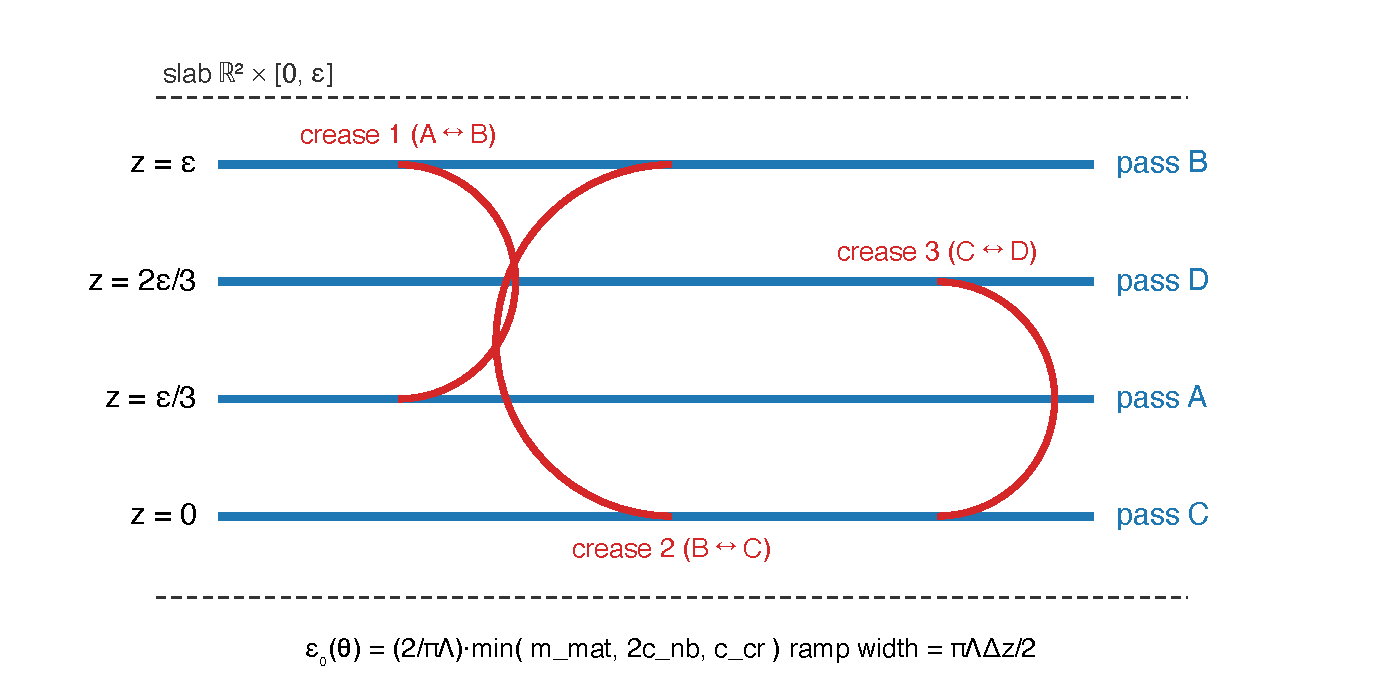
\includegraphics[width=0.9\linewidth]{figs/fig5-slab-ramp.pdf}
\caption{Strong $\varepsilon$-realization of an open state. The four passes are lifted to the constant heights $z_C=0<z_A=\varepsilon/3<z_D=2\varepsilon/3<z_B=\varepsilon$ dictated by the layer order $B>D>A>C$, and each crease is replaced by an isometric hairpin ramp \eqref{eq:hairpin} of radius $r_i$ and collar half-width $\pi r_i/2$. The slab budget $\varepsilon_0(\theta)$ of \eqref{eq:eps0} is exactly what keeps the three collision classes---sheet against sheet, ramp against sheet, ramp against ramp---disjoint.}
\label{fig:slab}
\end{figure}

\subsection{Tight states, necessity, and the equivalence}

Theorem~\ref{thm:openreal} does not apply to zero-clearance states, tight ones in particular: by Observation~\ref{obs:budget} a tight state has $\varepsilon_0=0$, so no room is left for ramps. The remedy is to open the state slightly and then pass to the limit.

\begin{lemma}[Opening]\label{lem:opening}
The pentagonal and dagger states are limits of open valid states with the same layer order. At $\td$ the four-by-four minor of the active-gradient matrix in the $(g,h,a,b)$ columns is exactly nonzero in $\Q[x]/(p_x)$, with value $-0.956\ldots$, so the system $\nabla w_j\cdot\delta=1$ for $j\in\{1,4,5,6\}$ has a solution $\delta$; at the pentagon the explicit rational direction
\begin{equation}\label{eq:openingdir}
  \delta^{\mathrm{op}}=\Bigl(-\tfrac{93}{1000},\ \tfrac{2197}{1000},\ \tfrac{1021}{500},\ \tfrac{509}{250},\ \tfrac{419}{200}\Bigr)
\end{equation}
has all eight wall derivatives rigorously positive, the eight values lying in the interval $[0.984,1.018]$.
\end{lemma}

\begin{proof}
The minor is computed by exact arithmetic in $\Q[x]/(p_x)$ and the interval range for \eqref{eq:openingdir} by interval arithmetic, both in the ancillary suite \cite{anc}. Given such a $\delta$, the walls and the material-consistency functions are rational, hence $C^1$, and the inactive constraints are strict at the tight state, so $w_j(\theta+t\delta)=t\,(\nabla w_j\cdot\delta)+O(t^2)>0$ for every wall and every small $t>0$: the perturbed states are valid and open, and they converge to the tight state as $t\downarrow0$.
\end{proof}

\begin{corollary}[Slack start at the pentagon]\label{cor:slackstart}
For all sufficiently small $t>0$ the state $q_t=P^*+t\,\delta^{\mathrm{op}}$ is slack: every wall satisfies $w_j(q_t)\ge0.98\,t+O(t^2)>0$ by \eqref{eq:openingdir}. The exact directional derivative is
\[
\begin{aligned}
\nabla\core(P^*)\cdot\delta^{\mathrm{op}}
 &=\frac12\left(-\frac{93}{1000}+\frac{2197}{1000}
                  +\frac{1021}{500}+\frac{509}{250}+\frac{419}{200}\right)\\
 &=\frac{8277}{2000}.
\end{aligned}
\]
Since $\core$ is affine on the forward chart,
\[
\core(q_t)=\core(P^*)+\frac{8277}{2000}\,t
\]
holds exactly. The reverse segment $s\mapsto q_{t-s}$, $0\le s\le t$, is therefore a pulling path from the slack state $q_t$ to $P^*$ with strictly decreasing core length. Concatenated with the certified monotone path of Remark~\ref{rem:edge}, this exhibits $\td$ as reachable from slack states, closing the reachability clause of Definition~\ref{def:pull}.
\end{corollary}
\begin{proof}
Positivity of the eight directional derivatives on the stated interval is the interval certificate of Lemma~\ref{lem:opening}; the gradient identity $\nabla\core(P^*)=\tfrac12\mathbf 1$ is Proposition~\ref{prop:gradpent}; the arithmetic is exact. Monotonicity of the concatenation is strict on each segment by the displayed rate and by Remark~\ref{rem:edge}.
\end{proof}

The general statement---that every valid closed state is a limit of open valid states, that is, that the valid set is the closure of its interior in the appropriate semialgebraic sense---is not proved here. Lemma~\ref{lem:opening} establishes exactly the two instances that the main theorems require.

\begin{theorem}[Limit realization of closed states]\label{thm:limitreal}
Let $\bar\theta$ be a valid state satisfying the axioms, with walls allowed to be active, and suppose $\bar\theta=\lim_k\theta_k$ for open valid states $\theta_k$ carrying the same layer order. Then $(f_{\bar\theta},\lambda)$ has a limit realization. In particular $\td$ and the regular pentagon do.
\end{theorem}

\begin{proof}
Take $\varepsilon_k=\frac12\min(\varepsilon_0(\theta_k),1/k)$ and let $F_k$ be the strong realization of Theorem~\ref{thm:openreal} at $\theta_k$. On a compact material set,
\[
  \sup\lvert\pi F_k-f_{\bar\theta}\rvert\le\tfrac\pi4\varepsilon_k+\sup\lvert f_{\theta_k}-f_{\bar\theta}\rvert\longrightarrow0 ,
\]
because $\theta\mapsto f_\theta$ is uniformly continuous on compacta: vertices and directions are rational functions of $\theta$ whose denominators stay bounded away from zero near a valid state. For the separation clause, a compact set $V$ at distance $d_0>0$ from the creases of $\bar\theta$ is at distance at least $d_0/2>C_{\mathrm{ram}}\varepsilon_k$ from the creases of $\theta_k$ for all large $k$, so the constant-height separation \eqref{eq:sheetsep} of $F_k$ applies on $V$, with the same $\lambda$ throughout the sequence. The routine verifications are carried out in the ancillary suite \cite{anc}.
\end{proof}

\begin{lemma}[Mod-2 crossing parity]\label{lem:mod2}
Let $U\subset\R^2$ be an open disc and let $W$ be a compact material region inside a single panel with $f|_W$ a homeomorphism, $\overline U\subset\operatorname{int}f(W)$, and $d(\overline U,\partial f(W))=3\delta_0>0$. Let $F$ be a piecewise $C^2$ embedding with $\sup_W\lvert\pi F-f\rvert<\delta_0$, and put $S=F(W)$. Then every vertical fibre over $U$ meets $S$, and a vertical segment in general position containing the whole $S$-part of its fibre has mod-2 intersection number one with $S$; consequently any piecewise $C^1$ path whose projection stays in $U$, beginning below the entire $S$-part of its fibre and ending above the entire $S$-part of its fibre, must meet $S$. The intersection-theoretic ingredients---transversality, homotopy invariance of the mod-$2$ intersection number for boundaryless targets, and its computation on a fibre---are the standard ones \cite{gp1974}.
\end{lemma}

\begin{proof}
For the first assertion, the straight homotopy $(1-\tau)\pi F|_W+\tau f|_W$ keeps $\partial W$ at distance at least $2\delta_0$ from $\overline U$, so $\deg_2(\pi F|_W,u)=\deg_2(f|_W,u)=1$ for every $u\in U$, and the mod-2 count of a segment covering the whole $S$-part of the fibre equals this degree. For the second, suppose the path $\alpha$ misses $S$, and close it into a cycle $\gamma$ inside the cylinder $\overline U\times\R$: run $\alpha$, rise vertically above the slab, cross horizontally at that height, and descend the initial fibre. The three added pieces contribute $0$, $0$ and, by the first assertion, $1$, so $\gamma\cdot S\equiv1\pmod2$. But $\partial S=F(\partial W)$ projects outside $\overline U$, so $\gamma$ contracts inside the cylinder through the complement of $\partial S$, whence $\gamma\cdot S\equiv\mathrm{lk}_2(\gamma,\partial S)\equiv0$---a contradiction.
\end{proof}

\begin{theorem}[Necessity]\label{thm:necessity}
If a state of the overhand branch has a limit realization, then it satisfies the crease-neighbourhood axiom of Definition~\textup{\ref{def:axiom}}.
\end{theorem}

\begin{proof}
Suppose the axiom fails: a pass $Q$ lying strictly between $P$ and $P'$ in the layer order covers a neighbourhood of an interior point $p_0$ of the crease joining $P$ and $P'$. Choose a short material segment $\sigma$ crossing that crease at $p_0$ whose image remains inside the covered neighbourhood, and perturb it into general position so that the images of its two endpoints avoid all three creases. Let $V_\pm$ be small \emph{fixed} discs about those two endpoint images, at positive distance from the creases and inside the relevant overlap regions. Because the discs are fixed, and not shrinking with $k$, the separation clause of Definition~\ref{def:limitreal} applies on them for all large $k$; it places $F_k(\sigma(-1))$ below and $F_k(\sigma(+1))$ above the entire $S$-part of their respective fibres, where $S=F_k(W)$ for a compact $W\subset Q$ lying over the relevant disc. Lemma~\ref{lem:mod2} then forces $F_k\circ\sigma$ to meet $S$, that is, forces two disjoint material sets to share an image, contradicting injectivity of $F_k$. The point of the argument is that separation is needed only \emph{near the endpoints} of $\sigma$, never at $p_0$ itself, where the crease makes separation impossible; and $\sigma$ may always be taken short enough for its endpoint discs to clear the creases, however small the violated neighbourhood. The routine verifications are carried out in the ancillary suite \cite{anc}.
\end{proof}

\begin{theorem}[Realization completeness for the globally ordered three-crease branch]\label{thm:completeness}
For states $(f_\theta,\lambda)$ of the globally ordered overhand branch $\mathcal B$ (fixing the total layer order $B>D>A>C$), with the opening hypothesis of Lemma~\textup{\ref{lem:opening}} imposed on states of zero clearance, the following are equivalent:
\begin{enumerate}
\item[(a)] the state satisfies the crease-neighbourhood axiom and crease-pair non-crossing (with respect to $B>D>A>C$);
\item[(b)] the state admits a limit realization by embeddings into $\R^2\times[0,\varepsilon_k]$ with $\varepsilon_k\downarrow0$ inducing the order $B>D>A>C$ in the sheet-separation sense.
\end{enumerate}
Here (a) implies (b) unconditionally for open states, and is there strengthened to strong $\varepsilon$-realizations for every $\varepsilon<\varepsilon_0(\theta)$; for states of zero clearance the implication holds under the opening hypothesis, which is certified for $\td$ and for the regular pentagon. The converse implication is unconditional within $\mathcal B$. By contrast, if $\lambda$ is allowed to be an arbitrary pointwise local order, then strong $\varepsilon$-realizability does not force a global total order \textup{(Remark~\ref{rem:cyclic-counterexample})}, though it does wherever all four passes share a common interior point \textup{(Lemma~\ref{lem:common-overlap})}.
\end{theorem}

\begin{proof}
For (a) implies (b): open states are covered by Theorem~\ref{thm:openreal}, and a strong $\varepsilon$-realization for all small $\varepsilon$ yields a limit realization on taking $\varepsilon_k=1/k$; states of zero clearance are covered by Theorem~\ref{thm:limitreal} together with Lemma~\ref{lem:opening}. For (b) implies (a): the crease-neighbourhood axiom is Theorem~\ref{thm:necessity}, and with the global layer order $B>D>A>C$ fixed in $\mathcal B$, the transversality clause of crease-pair non-crossing follows from Proposition~\ref{prop:axred}.
\end{proof}

Theorem~\ref{thm:completeness} is Theorem~\ref{mainthm:realization}.

\begin{remark}[What the axioms actually are]\label{rem:axiomreduction}
Within the globally ordered branch $\mathcal B$, Theorem~\ref{thm:completeness} and Proposition~\ref{prop:axred} separate the independent hypotheses: the crossing datum together with the global total order $B>D>A>C$ (which is forced locally by Lemma~\ref{lem:common-overlap} on the common-overlap locus, but not globally by Remark~\ref{rem:cyclic-counterexample}), and the crease-neighbourhood axiom, from which transverse crease-pair non-crossing follows. That the taco pair $w_9,w_{10}$ appears as a separate pair of walls is a matter of analytic signature rather than logical independence; geometrically, by Observation~\ref{obs:corner}, it is the corner contact of the crease pair $\kappa_1,\kappa_3$.
\end{remark}

\begin{remark}[Numerical remark]\label{rem:slabnumerics}
The clearance values behind Observation~\ref{obs:budget} are $c_{\mathrm{cr}}(\td)=0.0845$ and $m_{\mathrm{mat}}(\td)=1.036$ against $c_{\mathrm{nb}}(\td)=0$, while at the pentagon $c_{\mathrm{nb}}=c_{\mathrm{cr}}=0$ (\texttt{check\_realize}). Along the opening path $\theta_t=\td+t\delta$ of Lemma~\ref{lem:opening} one finds $c_{\mathrm{nb}}(\theta_t)\approx0.96\,t$ and $\varepsilon_0(\theta_t)\approx1.16\,t$, so realizing the state in a slab of fixed height $\varepsilon$ along this path costs an opening $t\gtrsim\varepsilon/1.16$, and then, using $\nabla w_j\cdot\delta=1$ and the multipliers of Theorem~\ref{thm:kkt},
\[
  \core(\theta_t)-\ell^\dagger=\Bigl(\sum_j\lambda_{w_j}\nabla w_j\cdot\delta\Bigr)t+O(t^2)
  =\Bigl(\sum_j\lambda_{w_j}\Bigr)t+O(t^2)\approx4.111\,t ,
\]
in agreement with the measured value $\core-\ell^\dagger=4.11\times10^{-3}$ at $t=10^{-3}$. Composing the two estimates gives $\core(\varepsilon)-\ell^\dagger\lesssim3.5\,\varepsilon$: this construction supplies nearby zero-thickness states in a slab of height $\varepsilon$ with an $O(\varepsilon)$ core-length cost. The coefficient combines the KKT multiplier sum with the chosen opening rate; it is not a material-thickness law or a prediction that physical pulling must stop there. This is an upper bound produced by one particular construction, and no matching lower bound is established, another slab realization possibly doing better. Two further points remain open: whether a state of zero clearance admits a \emph{strong} $\varepsilon$-realization at fixed small $\varepsilon$---the constant-height construction certainly fails there, and a wedge-shaped height assignment is the natural candidate---and the equivalence of the two forms of the induced layer order discussed in Remark~\ref{rem:sheetform}.
\end{remark}
